% generated by scripts/pkl_to_latex.py
% source PKL : excited_singlet_v1_L6_Ne6_U10_t1_mode-uniform_tpall_t2all_tperpall_nmin2_solver-gcg_sz0_restarts10_iter200_kmax4_tol1em09_cut10_adaptive1_step5_clusteravg1_T-none_knone_diag0.pkl
% scan type  : excited_singlet
% state      : ex_singlet
% requires   : \usepackage{pgfplots} \pgfplotsset{compat=1.18}
% colours match the matplotlib PDF (tab10 cycle)
\definecolor{gmeC0}{HTML}{1F77B4}
\definecolor{gmeC1}{HTML}{FF7F0E}
\definecolor{gmeC2}{HTML}{2CA02C}
\definecolor{gmeC3}{HTML}{D62728}
\definecolor{gmeC4}{HTML}{9467BD}
\definecolor{gmeC5}{HTML}{8C564B}
\definecolor{gmeC6}{HTML}{E377C2}
\definecolor{gmeC7}{HTML}{17BECF}

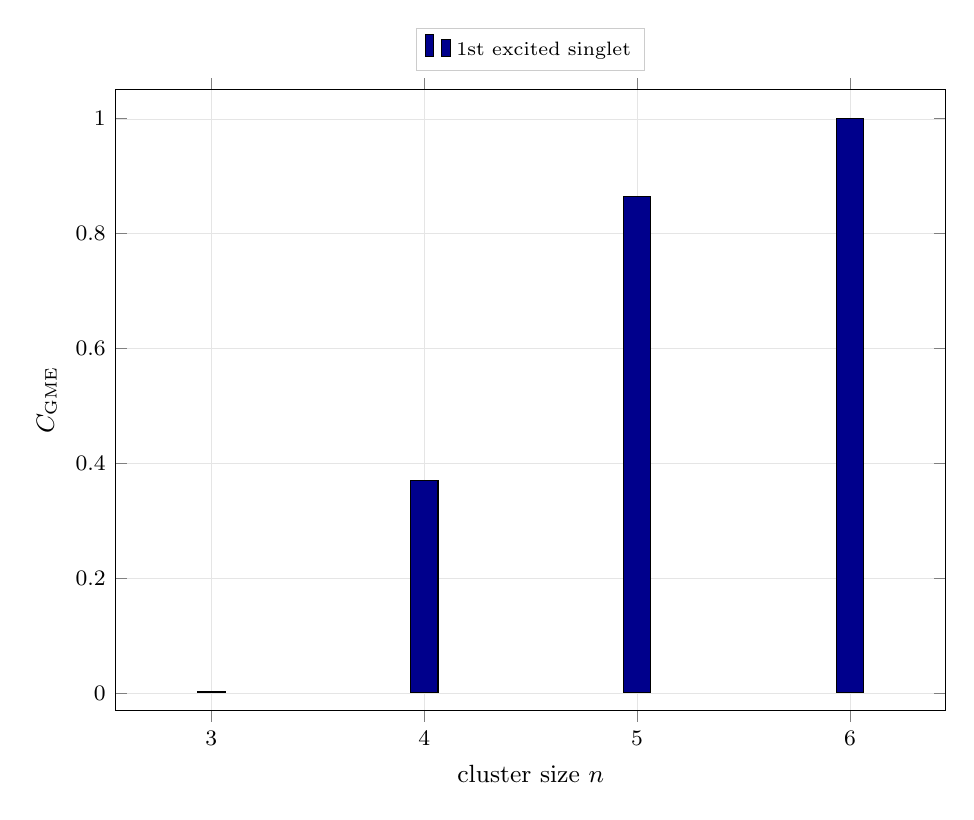
\begin{tikzpicture}
  \begin{axis}[
    width=\columnwidth,
    height=0.78\columnwidth,
    xlabel={cluster size $n$},
    ylabel={$C_{\mathrm{GME}}$},
    grid=both,
    grid style={line width=.1pt, draw=gray!20},
    tick label style={font=\footnotesize\rmfamily, /pgf/number format/fixed},
    label style={font=\small\rmfamily},
    scaled ticks=false,
    legend style={font=\scriptsize\rmfamily, draw=gray!40, at={(0.5,1.03)}, anchor=south, /tikz/every even column/.append style={column sep=6pt}},
    legend cell align={left},
    legend columns=1,
    ymin=-0.03,
    ymax=1.05,
    xtick={3,4,5,6}, ybar, enlarge x limits=0.15,
  ]
    \addplot[ybar, fill=blue!55!black, draw=black, bar width=10pt] coordinates {(3,0.003019) (4,0.370446) (5,0.864713) (6,1)};
    \addlegendentry{1st excited singlet}
  \end{axis}
\end{tikzpicture}

\begin{table}[htbp]
  \centering
  \caption{Spin classification of the lowest eigenstates of the $L=6$, $K=6$ Hubbard ring.}
  \label{tab:spin-l6-ne6-31d31f}
  \begin{tabular}{rrrrrl}
    \hline\hline
    Index & Energy & $\langle S^2\rangle$ & $S$ & $2S+1$ & Label \\
    \hline
    0 & -1.664363 & -0.0000 & 0.00 & 1 & Singlet (S=0) \\
    1 & -1.390497 & 2.0000 & 1.00 & 3 & Triplet (S=1) \\
    2 & -1.163673 & -0.0000 & -0.00 & 1 & Singlet (S=0) \\
    3 & -1.080001 & 2.0000 & 1.00 & 3 & Triplet (S=1) \\
    4 & -1.080001 & 2.0000 & 1.00 & 3 & Triplet (S=1) \\
    5 & -0.967248 & 2.0000 & 1.00 & 3 & Triplet (S=1) \\
    6 & -0.967248 & 2.0000 & 1.00 & 3 & Triplet (S=1) \\
    7 & -0.781279 & 0.0000 & 0.00 & 1 & Singlet (S=0) \\
    8 & -0.781279 & -0.0000 & -0.00 & 1 & Singlet (S=0) \\
    9 & -0.771276 & 6.0000 & 2.00 & 5 & Quintet (S=2) \\
    10 & -0.582576 & 6.0000 & 2.00 & 5 & Quintet (S=2) \\
    11 & -0.582576 & 6.0000 & 2.00 & 5 & Quintet (S=2) \\
    \hline\hline
  \end{tabular}
\end{table}
